%% For double-blind review submission, w/o CCS and ACM Reference (max submission space)
\documentclass[acmsmall,review,anonymous]{acmart}\settopmatter{printfolios=true,printccs=false,printacmref=false}
%% For double-blind review submission, w/ CCS and ACM Reference
%\documentclass[acmsmall,review,anonymous]{acmart}\settopmatter{printfolios=true}
%% For single-blind review submission, w/o CCS and ACM Reference (max submission space)
%\documentclass[acmsmall,review]{acmart}\settopmatter{printfolios=true,printccs=false,printacmref=false}
%% For single-blind review submission, w/ CCS and ACM Reference
%\documentclass[acmsmall,review]{acmart}\settopmatter{printfolios=true}
%% For final camera-ready submission, w/ required CCS and ACM Reference
%\documentclass[acmsmall]{acmart}\settopmatter{}


%% Journal information
%% Supplied to authors by publisher for camera-ready submission;
%% use defaults for review submission.
\acmJournal{PACMPL}
\acmVolume{2}
\acmNumber{ICFP} % CONF = POPL or ICFP or OOPSLA
\acmArticle{1}
\acmYear{2018}
\acmMonth{9}
\acmDOI{10.1145/nnnnnnn.nnnnnnn}
\startPage{1}

%% Copyright information
%% Supplied to authors (based on authors' rights management selection;
%% see authors.acm.org) by publisher for camera-ready submission;
%% use 'none' for review submission.
\setcopyright{none}
%\setcopyright{acmcopyright}
%\setcopyright{acmlicensed}
%\setcopyright{rightsretained}
%\copyrightyear{2018}           %% If different from \acmYear

%% Bibliography style
\bibliographystyle{ACM-Reference-Format}
%% Citation style
%% Note: author/year citations are required for papers published as an
%% issue of PACMPL.
\citestyle{acmauthoryear}   %% For author/year citations


%%%%%%%%%%%%%%%%%%%%%%%%%%%%%%%%%%%%%%%%%%%%%%%%%%%%%%%%%%%%%%%%%%%%%%
%% Note: Authors migrating a paper from PACMPL format to traditional
%% SIGPLAN proceedings format must update the '\documentclass' and
%% topmatter commands above; see 'acmart-sigplanproc-template.tex'.
%%%%%%%%%%%%%%%%%%%%%%%%%%%%%%%%%%%%%%%%%%%%%%%%%%%%%%%%%%%%%%%%%%%%%%


%% Some recommended packages.
\usepackage{booktabs}   %% For formal tables:
                        %% http://ctan.org/pkg/booktabs
\usepackage{subcaption} %% For complex figures with subfigures/subcaptions
%% http://ctan.org/pkg/subcaption

\usepackage[utf8]{inputenc}
\usepackage[T1]{fontenc}
\usepackage[scaled=0.85]{beramono}
\usepackage{amsmath}
\usepackage{amssymb}
\usepackage{xcolor,colortbl}
\usepackage{url}
\usepackage{listings}
\usepackage{paralist}
\usepackage{wrapfig}
\usepackage{enumitem}
\usepackage{multicol}
\usepackage{flushend}
\usepackage{tikz}

\usetikzlibrary{arrows,chains,matrix,positioning,scopes}
\makeatletter
\tikzset{join/.code=\tikzset{after node path={%
\ifx\tikzchainprevious\pgfutil@empty\else(\tikzchainprevious)%
edge[every join]#1(\tikzchaincurrent)\fi}}}
\makeatother

\tikzset{>=stealth',every on chain/.append style={join},
         every join/.style={->}}
\tikzstyle{labeled}=[execute at begin node=$\scriptstyle,
   execute at end node=$]

% ----- listings

\definecolor{ckeyword}{HTML}{7F0055}
\definecolor{ccomment}{HTML}{3F7F5F}
\definecolor{cstring}{HTML}{2A0099}

\lstdefinelanguage{Scala}%
{morekeywords={abstract,%
  sealed,%
  case,catch,char,class,%
  def,else,extends,final,finally,for,%
  if,import,implicit,%
  match,module,%
  new,null,undefined,%
  fun,array,
  override,%
  package,private,protected,public,%
  for,public,return,super,%
  this,throw,trait,try,type,%
  val,var,%
  with,while,%
  let,skip,assert,then,fst,snd,root,idx,sum,prod,exists,forall,%
  yield%
  },%
  sensitive,%
  moredelim=*[il][\bfseries]{\#\#\ },
  morecomment=[l]//,%
  morecomment=[s]{/*}{*/},%
  morestring=[b]",%
%  morestring=[b]',%
  showstringspaces=false%
}[keywords,comments,strings]%

\lstset{language=Scala,%
  mathescape=true,%
%  columns=[c]fixed,%
%  basewidth={0.5em, 0.40em},%
%  aboveskip=5pt,%\smallskipamount,
%  belowskip=5pt,%\negsmallskipamount,
  lineskip=0pt,
  basewidth={0.54em, 0.4em},%
%  backgroundcolor=\color{listingbg},
  basicstyle=\footnotesize\ttfamily,
  keywordstyle=\keywordstyle,
  commentstyle=\commentstyle,
  stringstyle=\stringstyle,
%  xleftmargin=0.5cm
  literate={-->}{{$\to$}}3 
           {->}{{$\mapsto$}}3 
           {=>}{{$\Rightarrow$}}2 
           {|-}{{$\ts$}}2 
           %{fun}{{$\lambda$}}1 
           {idx}{{$\#$}}1 
           %{sum}{{$\Sigma$}}1 
           {array(}{{$\langle.\rangle$(}}3 
           %{[[}{{$[\![$}}1
           %{]]}{{$]\!]$}}1
           %{…}{{$\!...$}}1 
}

\definecolor{listingbg}{RGB}{240, 240, 240}

\newcommand{\commentstyle}[1]{\color{ccomment}\itshape{#1}}
\newcommand{\keywordstyle}[1]{\color{ckeyword}\bfseries{#1}}
\newcommand{\stringstyle}[1]{\color{cstring}\bfseries{#1}}

\lstnewenvironment{listing}{\lstset{language=Scala}}{}
\lstnewenvironment{listingtiny}{\lstset{language=Scala,basicstyle=\scriptsize\ttfamily}}{}

\newcommand{\code}[1]{\lstinline[language=Scala,columns=fixed,basicstyle=\ttfamily]|#1|}


\newcommand{\IMP}[0]{\texttt{IMP}}
\newcommand{\FUN}[0]{\texttt{FUN}}

\newcommand{\TOOL}[0]{\texttt{SIGMA}}



% ----- packed items, so we don't waste space
\newenvironment{sitemize}{
\begin{itemize}
  \setlength{\itemsep}{1pt}
  \setlength{\parskip}{0pt}
  \setlength{\parsep}{0pt}
}{\end{itemize}}

\newenvironment{senumerate}{
\begin{enumerate}
  \setlength{\itemsep}{1pt}
  \setlength{\parskip}{0pt}
  \setlength{\parsep}{0pt}
}{\end{enumerate}}

\newcommand{\mypar}[1]{{\bf #1.}}

% ----- formal

%\newcommand{\judgement}[2]{{\bf #1} \hfill #2}
%\newcommand{\den}[1]{$\left\llbracket$\;#1\;$\right\rrbracket$}
\newcommand{\den}[1]{\llbracket~#1~\rrbracket}

%\newcommand{\ts}{\,\vdash\,}
\newcommand{\evalsto}{\Downarrow}

\newcommand{\mbind}{\;{\small{\texttt{>>}\hspace{-0.3pt}\raisebox{-0.15pt}{\texttt{=}}}}\;}

%\newcommand{\mbind}{{\small{\texttt{>>}\hspace{-1.7pt}\raisebox{-0.15pt}{\texttt{=}}}}}

\newcommand{\rref}[1]{\textsc{(#1)}}

% ----- comments and todo

\newcommand{\note}[1]{{\color{red}[#1]}}
\newcommand{\todo}[1]{\note{TODO: #1}}

\newcommand{\silent}[1]{}



\lstMakeShortInline[keywordstyle=,%
                    flexiblecolumns=false,%
                    %basewidth={0.56em, 0.52em},%
                    mathescape=false,%
                    basicstyle=\tt]@

\begin{document}

%% Title information
%\title{Pushdown Control Flow Analysis via Refunctionalization (Functional Pearl)}         %% [Short Title] is optional;
\title{Refunctionalization of Abstract Abstract Machines (Functional Pearl)}         %% [Short Title] is optional;
                                        %% when present, will be used in
                                        %% header instead of Full Title.
%\titlenote{with title note}             %% \titlenote is optional;
                                        %% can be repeated if necessary;
                                        %% contents suppressed with 'anonymous'
\subtitle{Filling the Gap Between Abstracting Abstract Machines and Abstracting Definitional Interpreters}        %% \subtitle is optional
%\subtitlenote{with subtitle note}       %% \subtitlenote is optional;
                                        %% can be repeated if necessary;
                                        %% contents suppressed with 'anonymous'


%% Author information
%% Contents and number of authors suppressed with 'anonymous'.
%% Each author should be introduced by \author, followed by
%% \authornote (optional), \orcid (optional), \affiliation, and
%% \email.
%% An author may have multiple affiliations and/or emails; repeat the
%% appropriate command.
%% Many elements are not rendered, but should be provided for metadata
%% extraction tools.

%% Author with single affiliation.
\author{First1 Last1}
\authornote{with author1 note}          %% \authornote is optional;
                                        %% can be repeated if necessary
\orcid{nnnn-nnnn-nnnn-nnnn}             %% \orcid is optional
\affiliation{
  \position{Position1}
  \department{Department1}              %% \department is recommended
  \institution{Institution1}            %% \institution is required
  \streetaddress{Street1 Address1}
  \city{City1}
  \state{State1}
  \postcode{Post-Code1}
  \country{Country1}                    %% \country is recommended
}
\email{first1.last1@inst1.edu}          %% \email is recommended

%% Author with two affiliations and emails.
\author{First2 Last2}
\authornote{with author2 note}          %% \authornote is optional;
                                        %% can be repeated if necessary
\orcid{nnnn-nnnn-nnnn-nnnn}             %% \orcid is optional
\affiliation{
  \position{Position2a}
  \department{Department2a}             %% \department is recommended
  \institution{Institution2a}           %% \institution is required
  \streetaddress{Street2a Address2a}
  \city{City2a}
  \state{State2a}
  \postcode{Post-Code2a}
  \country{Country2a}                   %% \country is recommended
}
\email{first2.last2@inst2a.com}         %% \email is recommended
\affiliation{
  \position{Position2b}
  \department{Department2b}             %% \department is recommended
  \institution{Institution2b}           %% \institution is required
  \streetaddress{Street3b Address2b}
  \city{City2b}
  \state{State2b}
  \postcode{Post-Code2b}
  \country{Country2b}                   %% \country is recommended
}
\email{first2.last2@inst2b.org}         %% \email is recommended


%% Abstract
%% Note: \begin{abstract}...\end{abstract} environment must come
%% before \maketitle command
\begin{abstract}
  Abstracting abstract machines (AAM) is a systematic methodology
  for constructing abstract interpreters that are derived from concrete
  small-step abstract machines. Recent progress applies the same idea
  on definitional interpreters, and obtains big-step
  abstract definitional interpreters (ADI) written in monadic style.
  Yet, the relations between small-step abstracting abstract machines and
  big-step abstracting definitional interpreters are not well studied.

  In this paper, we show their correspondence and how to syntactically transform small-step
  abstract abstract machines into big-step abstract definitional
  interpreters.
  The transformations include linearization, fusing, disentangling, refunctionalizing,
  and monadification (or un-CPS to direct-style). Linearization expresses
  non-deterministic choices by first-order data types, after which refunctionalization
  sequentializes the evaluation order by higher-order functions.
  All transformations properly handle the collecting semantics and the
  nondeterminism of abstract interpretation.
  %After each transformation, we also obtain an intermediate form of abstract interpreter.

  Following the idea that in deterministic languages
  evaluation contexts in reduction semantics are defunctionalized continuations,
  we further show that in nondeterministic languages, evaluation contexts are
  refunctionalized to extended continuations style.
  Remarkably, we reveal how precise call/return matching in control-flow
  analysis is obtained by refunctionalizing a small-step abstract
  abstract machine with proper caching.

  %As well as we explain how it been lost by defunctionalizing the higher-order continuations into an first-order data type.
\end{abstract}

%% 2012 ACM Computing Classification System (CSS) concepts
%% Generate at 'http://dl.acm.org/ccs/ccs.cfm'.
\begin{CCSXML}
<ccs2012>
<concept>
<concept_id>10011007.10011006.10011008</concept_id>
<concept_desc>Software and its engineering~General programming languages</concept_desc>
<concept_significance>500</concept_significance>
</concept>
<concept>
<concept_id>10003456.10003457.10003521.10003525</concept_id>
<concept_desc>Social and professional topics~History of programming languages</concept_desc>
<concept_significance>300</concept_significance>
</concept>
</ccs2012>
\end{CCSXML}

\ccsdesc[500]{Software and its engineering~General programming languages}
\ccsdesc[300]{Social and professional topics~History of programming languages}
%% End of generated code


%% Keywords
%% comma separated list
%\keywords{pushdown analysis, abstract interpretation, static analysis}  %% \keywords are mandatory in final camera-ready submission


%% \maketitle
%% Note: \maketitle command must come after title commands, author
%% commands, abstract environment, Computing Classification System
%% environment and commands, and keywords command.
\maketitle

\section{Introduction}

Defining a language by building an interpreter for it can be traced to the very
early time of programming languages research \cite{landin1966next, reynolds1972definitional}.
Nowadays, even an undergraduate student in computer science is able to build toy languages
through interpreters.
But building a sound abstract interpreter remains as an esoteric and difficult task until recent years.

\citeauthor{van2012systematic} proposed Abstracting Abstract Machines (AAM) methodology which can used
for constructing abstract interpreters of higher-order functional languages from concrete abstract machines
~\cite{van2012systematic, van2010abstracting}.
Given a concrete small-step abstract machine, (e.g, the CESK machine, Krivine's machine, etc.),
by allocating continuations in the store and bounding both the value addresses and continuation
addresses to be finite, we obtain an abstract interpreter with a finite state space which
can be used for performing sound static analysis.
One can further instantiate different polyvariant control flow analyses by using different address allocators \cite{Gilray:2016:ACP:2951913.2951936}.

Applying the same idea to big-step definitional interpreters, \citeauthor{darais2017abstracting}
built abstract definitional interpreters (ADI) that are written in monadic style \cite{darais2017abstracting}.
One of the advantages of a monadic interpreter is that it is modular and composable.
By changing the underlying monads, the definition of the interpreter is not modified,
but we can recover different semantics, including the concrete semantics and various
abstract semantics such as context-sensitivity and abstract garbage collection \cite{Sergey:2013:MAI:2491956.2491979}.

Broadly speaking, abstract abstract machines and abstract definitional 
interpreters are both some kind of abstract interpreters.
They are obtained by applying a combination of abstractions to their
concrete counterparts, abstract machines and definitional interpreters, respectively.
An interesting question would be how we can interderive these abstract semantics artifacts 
from the other one.

In the concrete world, the relations among reduction semantics, abstract machines,
definitional interpreters, and monadic interpreters is intensively studied by Danvy and his
collaborators in the past years
\cite{Ager:2003:FCE:888251.888254, Danvy:2001:DW:773184.773202, danvy2004refocusing, Danvy:2008:DIP:1411204.1411206, AGER2004223, ager2005functional, Danvy:2006:RW:2171265.2171268, danvy2009towards, biernacka2009towards}.
The abstract machines implement structural operational semantics in continuation style,
where the reduction contexts are defunctionalized continuations. One can derive definitional
interpreters by refunctionalizing the evaluation contexts of abstract machines,
and by defunctionalizing the higher-order functions, one may obtain abstract machines in the
reverse direction.

On the contrary, in terms of their abstract semantics artifacts,
the relations between small-step abstract abstract machines and big-step abstract
definitional interpreters, as well as the question of deriving one from the other is not
well-studied.
The fundamental difference between concrete semantics artifacts and abstract semantics
artifacts is nondeterminism. In addition to ensuring termination, abstract semantics
artifacts are usually equipped with a cache of explored state that is guaranteed to reach
the least fixed-point eventually.
In this functional pearl, we practically answer the question and relate AAM and ADI
by presenting a series of syntactical transformations on the program from
small-step abstract abstract machines to big-step abstract definitional interpreters.

In addition, the abstract abstract machines with unbounded stack naturally correspond
to abstract definitional interpreters. We show after refunctionalizing an AAM with unbounded
stack, and with the proper caching algorithm, the pushdown control-flow analysis can be
obtained.

\subsection{Contribution}

We begin by reviewing some background
necessary for this work in Section~\ref{background}, as well as introducing some of the basic
code structures used throughout the paper. We then address the main contribution of this
paper, which is the filling of the gap between small-step AAM and big-step ADI by developing a
series of systematic transformations. Those transformations are summarized here, with their
associated section:

\begin{itemize}
\item We show \textbf{linearization} in Section~\ref{linear}. By expressing the
  nondeterministic choices as a first-order data type, we linearize the execution
  of abstract abstract machines; the transition of machine states therefore becomes deterministic. Notably, this introduces another layer of controls that will also be refunctionalized later.

\item In Section~\ref{fusing}, we then present the \textbf{fusing} transformation.
  The fusing transformation simply combines the single-step function @step@ and the driving
  function into one, but keeps all the machine state representations.

\item Section~\ref{disen} discusses \textbf{disentangling}, which disassembles the fused AAM to be several individual functions, with each function handling one data type represented by a continuation.

\item \textbf{Refunctionalization} is shown in Section~\ref{refunc} which sequentializes
  the order of abstract execution by higher-order functions.
  For clarity, we first present the refunctionalized AAM without caching. We then adopt a different caching algorithm to guarantee the termination of abstract interpretation.
  In this section, we also review pushdown control-flow analysis and examine how computable
    and precise call/return matching is obtained through these transformations.

\item The last transformation we show is that of transforming the refunctionalized AAM
  to a \textbf{direct-style} interpreter (Section~\ref{directstyle}) by using delimited controls.

\end{itemize}

These transformations are used throughout the paper, with refunctionalization and
defunctionalization of abstract interpreters playing important roles for the call stack of
the analyzed language. By refunctionalization, the call stack of the analyzed language
is blended into the call stack of the defining language. This provides another perspective to
explain why \citeauthor{darais2017abstracting}'s abstract definitional interpreters
is able to extend the the pushdown control-flow property from its defining language.

We complete this paper by discussing related work in Section~\ref{sec:related}, followed by concluding thoughts in Section~\ref{sec:conclusion}.

% \subsection{Contributions}

% the essence of abstracting definitional interpreter.

% We summarize our contributions as follows:

% \begin{itemize}
% \item The main contribution of this paper is the filling of the gap
%   between small-step AAM and big-step ADI by developing a series of
%   systematic transformations.
%   We show that the correspondence between abstract
%   machines and interpreters exists not only in concrete semantics artifacts,
%   but also in abstract semantics artifacts.
%   Galois connection?
%   \note{JD: Section number?}

% \item A new understanding of pushdown control flow analysis by
%   refunctionalization.
%   We present an abstract interpreter obtained from refunctionalizing
%   a small-step abstracting abstract machine.
%   This abstract interpreter naturally exhibits the pushdown control-flow property,
%   as the refunctionalization forces us to sequentialize the
%   abstract execution.
%   We also analyze its correctness, soundness, and termination.

% \item Further, we show that defunctionalization and refunctionalization
%   of abstract interpreters play important roles for the call stack of the analyzed language.
%   Given this insight, we reveal precisely \emph{why} small-step AAM has no pushdown
%   control-flow property (without extra efforts), as well as explain
%   why ADI naturally extends pushdown control-flow property from its
%   defining language.

% \end{itemize}

% \subsection{Outline}

% \note{TR: can this be merged with contributions? (they currently lack section refs)}
% The remainder of this paper is organized as follows.
% We begin by describing the target language we will analyze in Section~\ref{background},
% including a concrete CESK machine as small-step operational semantics for it.
% We continue with a review of abstracting abstract machines (AAM) as an abstract interpretation
% counterpart of CESK machines. Following this, Section~\ref{linear} shows a conversion from the
% nondeterministic choices of closures to another layer of continuations,
% therefore linearizing the abstract execution.
% Section~\ref{fusing} then discusses fusing the driver and step functions to a single
% function.
% We further identify in Section~\ref{disen} the first-order data type representations of
% continuations, and disentangle the code blocks for dispatching data types to separate
% functions.
% Section~\ref{refunc} then represents the refunctionalized abstract abstract machines.
% In this section, the continuations represented by data types become higher-order
% functions.
% In Section~\ref{directstyle}, we transform the refunctionalized AAM to two
% different direct styles: one implemented with monads, the other using
% delimited controls.

% Finally, we discuss related work in Section~\ref{sec:related}, followed by concluding thoughts in Section~\ref{sec:conclusion}.

\note{TR: put this into a proper figure, add known danvy sequence
for concrete evaluators at the bottom (in grey or dashed lines)}

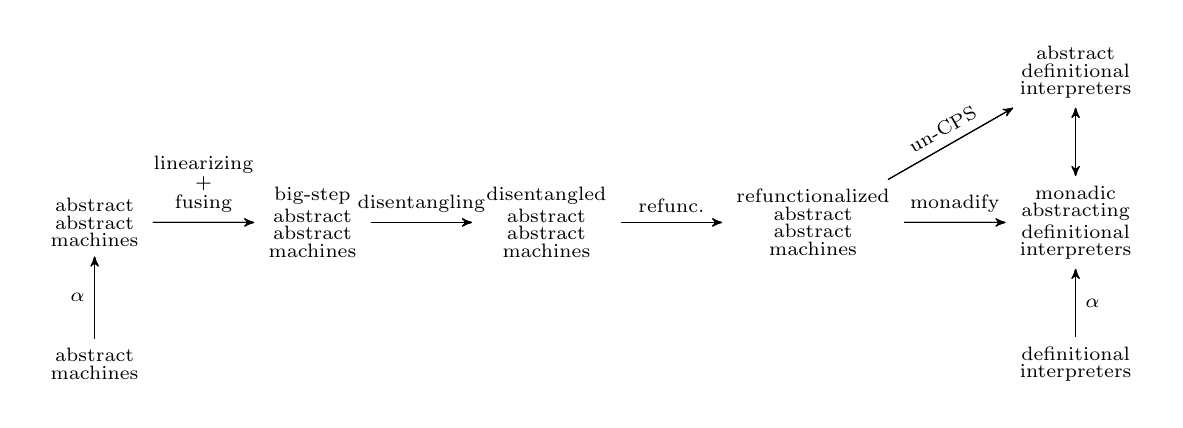
\begin{tikzpicture}
  \matrix (m) [matrix of math nodes, row sep=2.5em, column sep=3.7em]
    {
        &  &  &  &
      \begin{smallmatrix} \text{abstract} \\ \text{definitional} \\ \text{interpreters} \end{smallmatrix} \\
      \begin{smallmatrix} \text{abstract} \\ \text{abstract} \\ \text{machines} \end{smallmatrix} &
      \begin{smallmatrix} \text{big-step} \\ \text{abstract} \\ \text{abstract} \\ \text{machines} \end{smallmatrix}  &
      \begin{smallmatrix} \text{disentangled}  \\ \text{abstract} \\ \text{abstract} \\ \text{machines} \end{smallmatrix} &
      \begin{smallmatrix} \text{refunctionalized}  \\ \text{abstract} \\ \text{abstract} \\ \text{machines} \end{smallmatrix} &
      \begin{smallmatrix} \text{monadic} \\ \text{abstracting} \\ \text{definitional} \\ \text{interpreters} \end{smallmatrix}  \\
      \begin{smallmatrix} \text{abstract} \\ \text{machines} \end{smallmatrix} &
        &
      %\begin{smallmatrix} \text{big-step} \\ \text{abstract} \\ \text{machines} \end{smallmatrix}  &
        &
      %\begin{smallmatrix} \text{disentangled} \\ \text{abstract} \\ \text{machines} \end{smallmatrix} &
        &
      %\begin{smallmatrix} \text{refunctionalized} \\ \text{abstract} \\ \text{machines} \end{smallmatrix} &
      \begin{smallmatrix} \text{definitional} \\ \text{interpreters} \end{smallmatrix} \\
    };
  {
    [start chain] \chainin (m-2-4);
    \chainin (m-1-5) [join={node[sloped,anchor=center,above,labeled] {\text{un-CPS}}}];
    \chainin (m-2-5) [join={node[above,labeled] {\text{}}}];
    \chainin (m-1-5) [join={node[above,labeled] {\text{}}}];
  }
  {
    [start chain] \chainin (m-2-1);
    \chainin (m-2-2) [join={node[above,labeled] {\begin{smallmatrix} \text{linearizing} \\ \text{+} \\ \text{fusing} \end{smallmatrix}}     }];
    \chainin (m-2-3) [join={node[above,labeled] {\text{disentangling}}}];
    \chainin (m-2-4) [join={node[above,labeled] {\text{refunc.}}}];
    \chainin (m-2-5) [join={node[above,labeled] {\text{monadify}}}];
  }
  {
    [start chain]
    \chainin (m-3-1);
    { [start branch=A] \chainin (m-2-1)
      [join={node[left, labeled] {\alpha}}];
    }
  }
    %\chainin (m-2-2);
    %\chainin (m-2-3);
    %\chainin (m-2-4);
  {
    [start chain]
    \chainin (m-3-5);
    { [start branch=B] \chainin (m-2-5)
      [join={node[right, labeled] {\alpha}}];
    }
  }
\end{tikzpicture}

\iffalse
\subsection{Style}

We use Scala language to demonstrate the idea and each step of transformations.
We expect that readers have moderate familiarity to Scala's syntax, such as
case classes, pattern matching and for comprehension.

There are two main reasons we use a real-world language:
1) The code does not diminish the accuracy of the material
than formal and mathematical notations,
which are heavily used in other static analysis or semantics papers.
The Scala code in this paper can be easily back-translated into formal notations.
2) As a functional pearl, the code in this paper is executable with only few changes,
which make it particularly fit for presenting syntactical transformations on abstract
interpreters.
\fi

\section{Background} \label{background}

\subsection{A-Normal Form $\lambda$-Calculus} \label{anfsyntax}

Traditionally, continuation-passing style (CPS) is a popular intermediate representation
for analyzing functional programs because it exposes control transfer explicitly
and simplifies analysis~\cite{Shivers:1991:SSC:115865.115884, Shivers:1988:CFA:53990.54007}.
Here, we choose to use $\lambda$-calculus in administrative normal form (ANF) \cite{flanagan1993essence},
which is a direct-style intermediate representation, as our target for clarity,
but without losing simplicity and generality.
The transformations we will show in the rest of this paper
also work on abstract machines for plain direct-style $\lambda$-calculus languages.
Although we only show the core calculus language, it can be easily extended
to support recursive bindings (such as @letrec@), conditionals, primitive types, and
operations on primitive types. These cases would be trivial to implement,
so we elide them in this paper.

To begin, we present the concrete syntax of a call-by-value $\lambda$-calculus language
in ANF.

\begin{lstlisting}
    e $\in$ Exp ∂::= ae | (let ([x (ae ae)]) e)
   ae $\in$ AExp ::= ∂x | lam
  lam $\in$ Lam ∂::= (lambda (x) e)
    x $\in$ Var   (variable names)
\end{lstlisting}

In ANF, an expression is either an atomic expression or a @let@ expression.
A restriction exists which states that all function applications must be administrated
within a @let@ expression and then bound to a variable name under the current environment.
Both the operator and operand of function applications are atomic expressions.
An atomic expression $ae$ is either a variable or a literal @lambda@ term, either of which
can be evaluated in a single step.
We also assume that all the variable names in the program are unique.

The abstract syntax can be straightforwardly described in Scala as follows:
\note{TR: grammar below isn't ANF. Either make it so, or clarify that
we assume ANF only as convention and don't need/want to enforce it in
the term structure}

\begin{lstlisting}
sealed trait Expr
case class Var(x: String) extends Expr
case class App(e1: Expr, e2: Expr) extends Expr
case class Lam(x: String, body: Expr) extends Expr
case class Let(x: String, e: App, body: Expr) extends Expr
\end{lstlisting}

\subsection{CESK Machine} \label{cesk}

\subsubsection{Machine Components}

The CESK machine is an
abstract machine for describing semantics of and evaluating $\lambda$-calculus \cite{felleisen1987calculus}.
The CESK machine models program execution as state transitions in a small-step fashion.
As its name suggests, a machine state has four components:
1) \textit{Control} is the expression currently being evaluated.
2) \textit{Environment} is a map that contains the address of a variable in the lexical scope.
3) \textit{Store} models the heap of a program as a map from addresses to values.
The address space consists of numbers (0-indexed).
In our toy language, the only category of value is a closure, i.e., a function paired with an environment.
4) \textit{Continuation} represents the program stack. \todo{explain more on stack}

The Scala representations for the components of CESK machine are as follows:

\begin{lstlisting}
type Addr = Int
type Env = Map[String, Addr]
type Store = Map[Addr, Storable]

abstract class Storable
case class Clos(v: Lam, env: Env) extends Storable

case class Frame(x: String, e: Expr, env: Env)
type Kont = List[Frame]

case class State(e: Expr, env: Env, store: Store, k: Kont)
\end{lstlisting}

It is worth noting that the continuation class @Kont@ is defined as a list of
frames, where a frame can be considered an evaluation context in reduction semantics.
We represent frames using the @Frame@ class, which stores the information of a single
call-site, i.e., the information that can be used to resume the interrupted computation.
A @Frame@ constitutes a variable name @x@ to be bound later, a control expression
to which the program may resume, and its environment. \note{JD: someone check this and make sure I got it right}
\todo{mention that frame list vs KArg/KFun}

\subsubsection{Single-Step Transition}
Before describing how the machine evaluates expressions, we must first define several helper
functions. As mentioned in Section~\ref{anfsyntax}, atomic expressions are either a variable
or a literal @lambda@ term. As such, the atomic expression evaluator @atomicEval@ handles
these two cases and evaluates atomic expressions to closures in a straightforward way.
The @alloc@ function generates a fresh address, and always allocates a unique integer
in the domain of @store@.
The @isAtomic@ function is used as a predicate to determine if the expression is atomic.

\begin{lstlisting}
def atomicEval(e: Expr, env: Env, store: Store): Storable = e match {
  case Var(x) => store(env(x))
  case lam @ Lam(x, body) => Clos(lam, env)
}
def alloc(store: Store): Addr = store.keys.size + 1
def isAtomic(e: Expr): Boolean = e.isInstanceOf[Var] || e.isInstanceOf[Lam]
\end{lstlisting}

We can now faithfully describe the state transition function @step@,
which when given a machine state, determines its successor state.

\begin{lstlisting}
def step(s: State): State = s match {
  case State(Let(x, App(f, ae), e), env, store, k) if isAtomic(ae) =>
    val Clos(Lam(v, body), env_c) = atomicEval(f, env, store)
    val addr = alloc(store)
    val new_env = env_c + (v -> addr)
    val new_store = store + (addr -> atomicEval(ae, env, store))
    val frame = Frame(x, e, env)
    State(body, new_env, new_store, frame::k)
  case State(ae, env, store, k) if isAtomic(ae) =>
    val Frame(x, e, env_k)::ks = k
    val addr = alloc(store)
    val new_env = env_k + (x -> addr)
    val new_store = store + (addr -> atomicEval(ae, env, store))
    State(e, new_env, new_store, ks)
}
\end{lstlisting}

As shown and previously discussed, we examine the only two cases which the state may be.

\begin{itemize}

\item In the first @case@ statement shown in the previous code,
the control of the current state matches as a @Let@ expression, with its right-hand side a
function application.
By calling the @atomicEval@ evaluator, we obtain the closure for which the callee @f@ stands.
The successor state's control then transfers to the @body@ expression of the closure
with an updated environment and store. The new environment is extended
from the closure's environment and mapped from @v@ to a fresh address @addr@.
The new store is extended with @addr@ mapping to the value of @ae@,
which in turn is evaluated from @atomicEval@.
Finally, a new frame @frame@ is pushed onto the stack @k@, where
@frame@ contains the variable name @x@ at the left-hand position of the @Let@,
the body expression of @Let@, and the lexical environment of the body expression.

\item If the state is not a @Let@ expression, then it must be
an atomic expression, as seen in the above code. In this scenario,
we begin by extracting the top frame of all available continuations.
The control (i.e., an atomic expression) of the current state is the evaluated term
that is being bound to the variable @x@ from the top frame.
The environment and store are updated with @x@ mapping to the closure value of @ae@.
Finally, the successor state is transferred to expression @e@ from the top frame,
which is the body of a @Let@ expression, with the updated environment, store, and
the rest of the stack @ks@.

\end{itemize}

\subsubsection{Valuation}

To run the program, we first use the @inject@ function (below) to construct an initial machine
state given an expression @e@. The initial state contains an empty environment,
store, and stack.
\begin{lstlisting}
def inject(e: Expr): State = State(e, Map(), Map(), Nil)
\end{lstlisting}

The @drive@ function is then used to evaluate
to a final state by iteratively applying @step@ on the current state until a state is reached
ion which the control is an atomic expression and the continuation stack is empty.
Naturally, we can then extract the value from the final state at last.

\begin{lstlisting}
def drive(s: State): State = s match {
  case State(ae, _, _, Nil) if isAtomic(ae) => s
  case _ => drive(step(s))
}
def eval(e: Expr): State = drive(inject(e))
\end{lstlisting}

\subsection{Abstracting Abstract Machines} \label{aam}
Abstracting abstract machines (AAM) is a systematic methodology that derives sound
abstract interpreters for higher-order functional languages from concrete
abstract machines \cite{van2012systematic, van2010abstracting}.
An abstracting abstract machine implements computable abstract semantics which
approximates the runtime behaviors of programs.
Since the state space of concrete execution is possibly infinite,
the key insight of AAM approach when analyzing programs is to allocate both bindings
and continuations on the store, and then bound the addresses space to be finite.
Since each component of state is finite,
the abstracted machine-state space is also finite, and therefore computable.

In this section, we derive the abstracting abstract machine from concrete
CESK machines, and also show how to instantiate
useful $k$-call-sensitive control flow analysis.

\subsubsection{Machine Components}

Similar to CESK machines, the machine state of AAM has a control expression,
an environment, a store, and continuation, as well as a timestamp.
However, there are several notable differences between AAM's store and CESK machine's store.
In AAM, the store maps addresses to sets of values; it stores all possible values
for a particular address. As such, dereferencing addresses becomes nondeterministic.
Also, the store performs \emph{joining}, rather than overwriting, when updating elements.
Furthermore, the continuations are likewise allocated on the store instead of formed into a
linked list, and the continuations are in a state which then turns into a continuation
address.

For clarity, we divide the store into two separate stores: the binding stores @BStore@, and
the continuation store @KStore@.
The binding store maps binding addresses to sets of closure values, whereas the continuation
store maps continuation addresses to sets of continuations.
We then define a generic class @Store[K,V]@ that performs joining when updating elements
in a store (below). By parameterizing @Store[K,V]@ with @[BAddr, Storable]@ and
@[KAddr, Cont]@, we obtain @BStore@ and @KStore@, respectively.

We note that the \note{store? update function? can a store be monotonic?} is monotonic; it continuously grows and never shrinks. This property
guarantees that in analyzing the \note{update function? store? pick the right word}, a fixed point can always be reached.

\begin{lstlisting}
case class Store[K,V](map: Map[K, Set[V]]) {
  def apply(addr: K): List[V] = map(addr).toList
  def update(addr: K, d: Set[V]): Store[K,V] = {
    val oldd = map.getOrElse(addr, Set())
    Store[K, V](map ++ Map(addr -> (d ++ oldd)))
  }
  def update(addr: K, sd: V): Store[K,V] = update(addr, Set(sd))
}
type BStore = Store[BAddr, Storable]
type KStore = Store[KAddr, Cont]
\end{lstlisting}

The codomain of all binding stores @Storable@ is the same
as previously defined for CESK machines.
The codomain of continuation stores @Cont@, on the other hand, is comprised of
a @Frame@ object and a continuation address @KAddr@.
To mimic the runtime call stack, @KAddr@ plays the role of
representing the remaining stack frames.
\todo{talk about nondet of cont deref?}

\begin{lstlisting}
abstract class Storable
case class Clos(v: Lam, env: Env) extends Storable

case class Frame(x: String, e: Expr, env: Env)
case class Cont(frame: Frame, kaddr: KAddr)
\end{lstlisting}

As a consequence, the components of states are also changed:
the store is divided into binding stores and continuation stores;
the continuation stack becomes an address.
By dereferencing this address in a continuation store, we can retrieve the
actual transfer of controls. The definition of environment @Env@
remains the same.

\begin{lstlisting}
case class State(e: Expr, env: Env, bstore: BStore, kstore: KStore, k: KAddr, time: Time)
\end{lstlisting}

\subsubsection{Allocating Addresses}
Up to this point, we have not described allocating addresses in stores,
nor handling the time stamp @Time@.
In abstract interpretation, however, these are key ingredients to achieve
analyses with different sensitivities, as well as to perform a finite
state space analysis\cite{Gilray:2016:ACP:2951913.2951936}.
To effectively approximate the runtime behavior, we introduce a finite
program counter @time@ that encodes the program execution history.
We use a list of execution contexts (expressions) to represent this, and
as we will see in Section~\ref{kcfainst}, by applying different @tick@
functions on the timestamp, we are able to obtain a family of analyses.

\begin{lstlisting}
type Time = List[Expr]
\end{lstlisting}

As previously mentioned, the space of addresses must be finite in AAM.
Binding addresses are parameterized by variable names and the creation time of the binding,
both of which are finite.
Continuation addresses @KAddr@ has two variants:
1) @Halt@ which corresponds to the empty stack, and
2) @ContAddr@ consists of the entry expressions of callee, which are also
finite.
One may ask, why not also keep track of the time in continuation addresses?
\todo{why target expression, allocation polyvariance}

\begin{lstlisting}
case class BAddr(x: String, time: Time)

abstract class KAddr
case object Halt extends KAddr
case class ContAddr(tgt: Expr) extends KAddr
\end{lstlisting}

We introduce two helper functions, @allocBind@ and @allocKont@, which will be
used to allocate binding addresses and continuation addresses.

\begin{lstlisting}
def allocBind(x: String, time: Time): BAddr = BAddr(x, time)
def allocKont(tgtExpr: Expr): KAddr = ContAddr(tgtExpr)
\end{lstlisting}

\subsubsection{Single-Step Transition}

Since dereferencing an address becomes nondeterministic, our @atomicEval@
function (below) is also nondeterministic. Given an atomic expression @e@,
@atomicEval@ returns a set of storable values (i.e., closures) to the caller.
If the expression is simply a @lambda@ term, the returned set is a singleton.

\begin{lstlisting}
def atomicEval(e: Expr, env: Env, bstore: BStore): Set[Storable] = e match {
  case Var(x) => bstore(env(x))
  case lam@Lam(x, body) => Set(Clos(lam, env))
}
\end{lstlisting}

The structure of function @step@ is similar to the concrete CESK machine,
except the nondeterminism which makes @step@ return a list of reachable successor states.
We have two cases to consider (code shown below):

\begin{itemize}
  \item If the current control expression is a @Let@, then
the result of @App(f, ae)@ will be bound to variable @x@. In this case, we retrieve the set
of closures that @f@ may represent. For each closure in the set, we perform nearly the same
operations as in the concrete CESK machines, with an important difference: the
continuation is allocated on the store @kstore@, so a new continuation address @new_kaddr@
must be constructed and a new frame @Frame(x, e, env)@ paired with the current continuation
address @kaddr@ is merged into @new_kaddr@. Finally, a list of successor states is generated.

  \item In the second case, an atomic expression @ae@ sits on the control position of the
state. Here, the value of @ae@ is being returned to its caller.
In order to accomplish this, we dereference the continuation address @kaddr@ and obtain a set
of continuations @conts@. For each continuation in the set, we construct an environment based
on the environment @env_f@ of the frame, and bind @x@ to a newly created binding address
@baddr@. We must also update the store with @baddr@ and the values that @ae@ represents. In
every generated state, the control becomes the expression @e@ in the frame, and as we can
tell from the name, the continuation address @f_kaddr@ also comes from the frame.
\end{itemize}

\begin{lstlisting}
def step(s: State): List[State] = {
  val new_time = tick(s)
  s match {
    case State(Let(x, App(f, ae), e), env, bstore, kstore, kaddr, time) =>
      val closures = atomicEval(f, env, bstore).toList
      for (Clos(Lam(v, body), env_c) <- closures) yield {
        val baddr = allocBind(v, new_time)
        val new_env = env_c + (v -> baddr)
        val new_bstore = bstore.update(baddr, atomicEval(ae, env, bstore))
        val new_kaddr = allocKont(body)
        val new_kstore = kstore.update(new_kaddr, Cont(Frame(x, e, env), kaddr))
        State(body, new_env, new_bstore, new_kstore, new_kaddr, new_time)
      }
    case State(ae, env, bstore, kstore, kaddr, time) if isAtomic(ae) =>
      val conts = kstore(kaddr).toList
      for (Cont(Frame(x, e, env_f), f_kaddr) <- conts) yield {
        val baddr = allocBind(x, new_time)
        val new_env = env_f + (x -> baddr)
        val new_store = bstore.update(baddr, atomicEval(ae, env, bstore))
        State(e, new_env, new_store, kstore, f_kaddr, new_time)
      }
  }
}
\end{lstlisting}

\subsubsection{$k$-Call-Sensitive Instantiation} \label{kcfainst}

In $k$-call-sensitive analysis, a history of the last $k$ call sites is
used as a finite program counter.
The history is represented as a list of expressions and embedded
in the allocated addresses.

Before transferring to successor states, we must use the @tick@ function to
refresh the timestamp, and then use this new timestamp for successors when allocating addresses.
The @tick@ function returns the $k$ front-most expressions given the current state and its
time history.

\begin{lstlisting}
def k: Int = 0
def tick(s: State): Time = (s.e :: s.time).take(k)
\end{lstlisting}

If we instantiate $k$ to be $0$, the history degenerates to an empty list,
and we obtain a monovariant analysis (i.e., it does
not differentiate values at different call sites). In this case, the address
space collapses to the space of variable names.
Note that regarding the ambiguity in $k$-CFA\cite{Gilray:2016:ACP:2951913.2951936},
the code here actually implements call+return \note{call+return, call/return, etc.? Check this} sensitivity.

\subsubsection{Collecting Semantics}

Similar to the CESK machines, to run (analyze) a program
we first use the @inject@ function to construct the initial state given to the program.
Note that the initial continuation store has a built-in mapping that maps the continuation
address for @Halt@ to an empty set of continuations.
We also provide an empty program counter as our initial time.
\begin{lstlisting}
def inject(e: Expr): State =
  State(e, Map(),
        Store[BAddr, Storable](Map()),
        Store[KAddr, Cont](Map(Halt -> Set())),
        Halt, List())
\end{lstlisting}

However, in contrast to the concrete CESK machine, the
@drive@ function performs collecting semantics instead of the valuation
semantics. That is, for the purpose of analyzing programs, the function @drive@
collects all the intermediate machine states as the program is abstractly executing.
The following code shows a variant of the worklist algorithm to find the fixed-point
of the set of states.\note{JD: I changed all of this to worklist instead of work list in favor of the worklist algorithm. Change this back if it's wrong.}
Function @drive@ always applies function @step@ to the head element @hd@ of
the worklist @todo@ if @hd@ is unseen. It then inserts the result of @step@ to
the rest of worklist, and in the meantime adds @hd@ to the explored states set.
If the worklist is empty, @drive@ simply returns the set of reachable states
up to the current execution point.

\begin{lstlisting}
def drive(todo: List[State], seen: Set[State]): Set[State] = todo match {
  case Nil => seen
  case hd::tl if seen.contains(hd) => drive(tl, seen)
  case hd::tl => drive(step(hd).toList ++ tl, seen + hd)
}

def analyze(e: Expr): Set[State] = drive(List(inject(e)), Set())
\end{lstlisting}

Finally, a user may invoke the @analyze@ function to obtain all reachable states for a given
program.

%\subsection{Monadic Abstract Interpreter}
%Maybe not here?

\subsection{One Step Back: Unabstracted Stack}

In this section, we describe a variant of AAM that allows the stack to be
unbounded which uses a precise call stack as we did in the concrete CESK machine.
Instead of allocating continuations in the store and embedding
addresses of continuations in states, we intend to use a list of frames
to explicitly model the stack.
By doing so, we recover the call stack as precise as runtimes
(so called pushdown control flow analysis), but since
the stack is unbounded, the analysis is potentially not computable.
For readers who are not familiar with pushdown analysis, we have a detailed
discussion in Section~\ref{pdcfarevisit}.
The reason we show it here is to establish an artifact with precise call/return matching
used for the next step of transformation.

In the definition of @State@, the continuation store disappears, and
component @konts@ becomes a list of frames. The other components remain unchanged.

\begin{lstlisting}
case class State(e: Expr, env: Env, bstore: BStore, konts: List[Frame], time: Time)
\end{lstlisting}

The state transition function @step@ shown below is still
nondeterministic, but the only nondeterminism happening is when dereferencing the callee @f@
from the function application @App(f, ae)@.

\begin{lstlisting}
def step(s: State): List[State] = {
  val new_time = tick(s)
  s match {
    case State(Let(x, App(f, ae), e), env, bstore, konts, time) if isAtomic(ae) =>
      for (Clos(Lam(v, body), env_c) <- atomicEval(f, env, bstore).toList) yield {
        val frame = Frame(x, e, env)
        val baddr = allocBind(v, new_time)
        val new_env = env_c + (v -> baddr)
        val new_store = bstore.update(baddr, atomicEval(ae, env, bstore))
        State(body, new_env, new_store, frame::konts, new_time)
      }
    case State(ae, env, bstore, konts, time) if isAtomic(ae) =>
      konts match {
        case Nil => List()
        case Frame(x, e, env_f)::konts =>
          val baddr = allocBind(x, new_time)
          val new_env = env_f + (x -> baddr)
          val new_store = bstore.update(baddr, atomicEval(ae, env, bstore))
          List(State(e, new_env, new_store, konts, new_time))
      }
  }
}
\end{lstlisting}

In the first case of pattern matching, we may have multiple choices of closure for callee @f@.
For each closure in the set, a new frame is constructed and pushed onto the stack.
The code for handling the second case (atomic expressions) is the same as the concrete CESK
machines.

\textbf{Note on Computability.}
Unfortunately, even though other components in the states are finite,
this AAM with an unbounded stack is still not computable.
This is because the unbounded stack can grow to arbitrary depth which implies that the state
space is possibly infinite; the analysis may therefore not terminate for all programs if we
simply enumerate reachable states. To see this, consider a program that has two mutually
recursive functions:

\begin{lstlisting}
(letrec ([f1 (lambda (x)
               (let ([x1 (f2 x)]) x1))]
         [f2 (lambda (y)
               (let ([y1 (f1 y)]) y1))])
  (let ([z (f1 1)])
    z))
\end{lstlisting}

Function @f1@ and @f2@ mutually invoke each other, so the stack will
alternate pushing frames @f1@ and @f2@ onto the top of current stack.
However, no two existing stack components are identical in the state space.

\section{Linearization} \label{linear}

In the previous section, we show that by keeping an unabstracted stack in the state
space, we can recover the precise call/return match.
In this and following sections, we begin describing the transformations step by step.
Our base machine for now is the AAM with unbounded stack, though
as we will later transform the stack to higher-order functions
represent \note{``representing'' or ``represented by''?} continuations, it does not matter what kind of AAM we start from.
This is because transforming to higher-order functions forces us to sequentialize
the order of abstract evaluation, and neither versions of AAM requires construction of a frame of lists \note{should this be frame of lists? sounds weird}, nor to allocate continuations in the store.
Thus, our choice to start from an AAM with unbounded stack is motivated simply because it has an equivalent stack model to abstract definitional interpreters (our final target).

\todo{Unbounded Stack AAM is PD, justify this}

In Danvy's paper \textit{Defunctionalized Interpreters for Programming
  Languages}, he mentioned for deterministic languages, a reduction semantics
is a structural operational semantics in continuation style, where the reduction
context is a defunctionalized continuation \cite{Danvy:2008:DIP:1411204.1411206}.
Here we are facing a problem:
the underlying semantics of AAM is fundamentally nondeterministic.
But the evaluation context (the @Frame@ in our program) is not
nondeterministic, and the work list @todo@ actually implicitly handles the nondeterminism,
if we simply refunctionalize the frames to functions, it would not helps toward
abstract definitional interpreters.

In order to address this problem, our first step of transformations
is to linearize all the nondeterministic choices.
This step turns the @step@ function to be deterministic.
Likewise the @Frame@ saves the information of the caller in concrete executions,
we introduce another layer of controls, and define a case class @NDCont@
that saves the information at a fork point when we have multiple target closures.
We also add a new field @ndk@ to the definition of state which is called
@NDState@ now.
For the rest of the paper, to differentiate the two continuations, we would call
the first one as normal continuation, and the second one as nondeterministic
continuations.

\begin{lstlisting}
case class NDCont(cls: List[Clos], argvs: Set[Storable], store: BStore, time: Time, frames: List[Frame])
case class NDState(e: Expr, env: Env, bstore: BStore, konts: List[Frame], time: Time, ndk: List[NDCont]) {
  def toState: State = State(e, env, bstore, konts, time)
}
\end{lstlisting}

A @NDCont@ contains a list of closures that are possible functions to be invoked,
a set of values that will be bind to the function's formal argument,
and the store, time, and frames at the fork point.
In the definition of @NDState@, an auxiliary function @toState@ is added that
converts itself to @State@.

Now the type of function @step@ becomes @NDState => NDState@.
The following code shows the first case of matching an instance of @NDState@ in
the @step@.

\begin{lstlisting}
case NDState(Let(x, App(f, ae), e), env, bstore, konts, time, ndk) =>
  val closures = atomicEval(f, env, bstore).toList.asInstanceOf[List[Clos]]
  val Clos(Lam(v, body), c_env) = closures.head
  val frame = Frame(x, e, env)
  val new_frames = frame::konts
  val baddr = allocBind(v, new_time)
  val new_env = c_env + (v -> baddr)
  val argvs = atomicEval(ae, env, bstore)
  val new_store = bstore.update(baddr, argvs)
  val new_ndk = NDCont(closures.tail, argvs, bstore, new_time, new_frames)::ndk
  NDState(body, new_env, new_store, new_frames, new_time, new_ndk)
\end{lstlisting}

By atomically evaluating @f@, we obtain a set of closures.
The transition is deterministic to the first element of the closure set.
So we just prepare new environment, new store, and new frame list only for the
first closure in that set.
A new nondeterministic continuation @new_ndk@ is also constructed,
which contains the rest of closures, the values of argument @ae@, the store,
the time and the new frame list.
We use the store before updating because for different closures they may form
different binding addresses @baddr@.
We also use the new frames, because all the closures at this fork point share
the same stack and return point.

In the second case shown in below we will see how @NDCont@ deal with
the nondeterminism.

\begin{lstlisting}
case NDState(ae, env, bstore, konts, time, ndk) if isAtomic(ae) =>
  konts match {
    case Nil => ndk match {
      case NDCont(Nil, _, _, _, _)::ndk =>
        NDState(ae, env, bstore, konts, time, ndk) /* transfer to the most recent fork point */
      case NDCont(cls, argvs, bstore, time, frames)::ndk =>
        val Clos(Lam(v, body), c_env) = cls.head
        val baddr = allocBind(v, time)
        val new_env = c_env + (v -> baddr)
        val new_store = bstore.update(baddr, argvs)
        val new_ndk = NDCont(cls.tail, argvs, bstore, tile, frames)::ndk
        /* resume the fork point with the next closure */
        NDState(body, new_env, new_store, frames, time, new_ndk)
    }
    case Frame(x, e, f_env)::konts =>
      val baddr = allocBind(x, newTime)
      val new_env = f_env + (x -> baddr)
      val new_store = bstore.update(baddr, atomicEval(ae, env, bstore))
      NDState(e, new_env, new_store, konts, newTime, ndk) /* normal return */
  }
\end{lstlisting}

If the normal continuation @konts@ is an empty list, then it means we have reached
the halt of computation; otherwise, we should return the values of @ae@ to its
caller which is contained in the top frame of stack.

But, since we have added nondeterminism into state, an empty list of frames means
we have the reached the halt of \textit{one computation path}, and we should
determine the next state indicates by @NDCont@.
So we have a pattern matching on @ndk@:
\begin{itemize}
  \item If the closure set is an empty set,
then we had tried all the closures of this fork point and should move the the
next fork point. Since the @NDCont@ is represented by a list and we always
append new element from its front, we are resuming to the most recent fork point by
popping up the front-most element.
\item Otherwise, we pop a closure from the set, then build new
environment and new store for the body expression of the closure;
we use the same frame list and time that are copied from the fork point rather
than current one.
The nondeterminism continuation @new_ndk@ is also updated by removal of that closure.
\end{itemize}

\begin{lstlisting}
def drive(nds: NDState, seen: Set[State]): Set[State] = {
  nds match {
    case NDState(ae, _, _, Nil, _, Nil) if isAtomic(ae) => seen
    case nds =>
      val s = nds.toState
      if (seen.contains(s)) drive(step(nds), seen)
      else drive(step(nds), seen + s)
  }
}
\end{lstlisting}

The function @drive@ is also changed: there is no work list anymore, because all the
potentially unexplored states are embedded in to the continuation for
nondeterminism.
The termination of the analysis is when we reach a @NDState@ that the expression
is atomic, and both the normal continuation and nondeterminism continuation are
empty list. This corresponds to the case that @todo@ list is empty.

Now, we obtain a linearized abstract abstract machine. If we image that the classical
AAM explores a graph of reachable states, then the linearized AAM just flattens the
graph to a linear sequence.

\section{Fusing} \label{fusing}

Fusing is a transformation that combines function @step@ and @drive@ to one.
The fused function @drive_step@ basically formed by merging function
@step@ into function @drive@.
@drive_step@ takes a @NDState@ and a set of explored states as argument,
and returns a set of reachable states once terminates.

\begin{lstlisting}
def drive_step(nds: NDState, seen: Set[State]): Set[State] = {
  nds match {
    case NDState(ae, _, _, Nil, _, Nil) if isAtomic(ae) => seen
    case nds =>
      val s = nds.toState
      val new_seen = if (seen.contains(s)) seen else seen+s
      val newTime = tick(nds)
      val new_ndstate = nds match {
        case NDState(Let(x, App(f, ae), e), env, bstore, konts, time, ndkonts) =>
          ......
        case NDState(ae, env, bstore, konts, time, ndkonts) if isAtomic(ae) =>
          ......
      }
      drive_step(new_ndstate, new_seen)
  }
}
\end{lstlisting}

Now we have a single function to perform both abstract evaluation and intermediate
states collecting. Given @inject(e)@ as the initial state and an empty set as
initial reached set, we can easily define the entrance function @analyze@ as follow.

\begin{lstlisting}
def analyze(e: Expr): Set[State] = drive_step(inject(e), Set())
\end{lstlisting}

\section{Disentangling} \label{disen}

In the last section, the fused AAM combines all the functions into one and
looks like a ``big-step'' interpreter, although it still has the machine
state representation inside.
In the disentangling transformation, we
identify the first-order data type represented evaluation contexts,
and lift the code blocks that handles these evaluation contexts to be individual functions.

Since there are two layers of continuations, as a result,
we obtain three mutually recursive functions, @drive_step@,
@continue@ and @ndcontinue@. The function @drive_step@ plays the same
role as before; @continue@ handles the evaluation context (@Frame@) of the analyzed
language, which the function is called from @drive_step@ when encountering an atomic
expression; @ndcontinue@ dispatches nondeterministic continuations @NDCont@,
and is invoked from @continue@ when the normal stack is empty.

\begin{lstlisting}
def drive_step(nds: NDState, seen: Set[State]): Set[State] = {
  nds match {
    case NDState(ae, _, _, Nil, _, Nil) if isAtomic(ae) => seen
    case nds =>
      val s = nds.toState
      val new_seen = if (seen.contains(s)) seen else seen + s
      val new_time = tick(nds)
      nds match {
        case NDState(Let(x, App(f, ae), e), env, bstore, konts, time, ndk) =>
          ......
          drive_step(NDState(body, new_env, new_store, new_frames, new_time, new_ndk), new_seen)

        case NDState(ae, env, bstore, konts, time, ndk) if isAtomic(ae) =>
          continue(nds, new_seen)
      }
  }
}
\end{lstlisting}

The above code shows the skeleton of function @drive_step@.
In the first case of pattern matching, the code for constructing new
environment, store and frames is omitted.
At the end of this case, we invoke @drive_step@ recursively.
The code for the second case is replaced by a function call to @continue@.
Now a vague shape of interpreter in continuation style is emerged.

\begin{lstlisting}
def continue(nds: NDState, seen: Set[State]): Set[State] = {
  val NDState(ae, env, bstore, konts, time, ndk) = nds
  val new_time = tick(nds)
  konts match {
    case Nil => ndcontinue(nds, seen)
    case Frame(x, e, f_env)::konts =>
      val baddr = allocBind(x, new_time)
      val new_env = f_env + (x -> baddr)
      val new_store = bstore.update(baddr, atomicEval(ae, env, bstore))
      drive_step(NDState(e, new_env, new_store, konts, new_time, ndk), seen)
  }
}
\end{lstlisting}

The function @continue@ is largely what we have for the second case in
@drive_step@, except a function call to @ndcontinue@ is placed when
the the normal continuation is empty.
Since we are analyzing a language in ANF, the first-order data representation of
continuation is simplified to @List@.
An empty list @Nil@ represents the halt of a computation path.
A cons @::@ means the top frame of the list holds the binding variable, and
evaluation context.
An analogue to this in standard CEK machines would be an abstract class (e.g., @cont@) with three
variants @halt@, @arg(value, cont)@ and @arg(exp, env, cont)@.

\begin{lstlisting}
def ndcontinue(nds: NDState, seen: Set[State]): Set[State] = {
  val NDState(ae, env, bstore, konts, time, ndk) = nds
  ndk match {
    case NDCont(Nil, _, _, _, _)::ndk =>
      drive_step(NDState(ae, env, bstore, konts, time, ndk), seen)
    case NDCont(cls, argvs, bstore, time, frames)::ndk =>
      val Clos(Lam(v, body), c_env) = cls.head
      val baddr = allocBind(v, time)
      val new_env = c_env + (v -> baddr)
      val new_store = bstore.update(baddr, argvs)
      drive_step(NDState(body, new_env, new_store, frames, time,
                         NDCont(cls.tail, argvs, bstore, time, frames)::ndk),
                 seen)
  }
}
\end{lstlisting}

The shape for function @ndcontinue@ is similar to function @continue@, after
all, they both use @List@ as a representation of continuations.
When the closure set is empty, we recursively call @drive_step@ with the rest
of @ndk@, since in this case the normal stack @konts@ is still empty, so
the state will be dispatched to @ndcontinue@ again.
Otherwise, we invoke @drive_step@ with the body expression of the next closure object.

\section{Refunctionalization} \label{refunc}

Refunctionalization transforms first-order data type represented
evaluation contexts to higher-order functions.
Besides sequentializing the order of abstract evaluation by functions,
this transformation can be also regarded as allocating continuation functions of
the defined language in the heap of the meta language.

In this section, several other notable changes have been made:
\begin{itemize}
\item We do not have the concept of @state@ (or @NDState@) anymore.
  The components of the states are lifted as arguments of the evaluation
  function.
\item Since our final target is abstract definitional interpreters while still
nondeterministic, start from this section, our abstract semantic artifact
returns a set of final values instead of collected states.
\item As we are getting close to the
abstract definitional interpreters, the name of @drive_step@ is updated to
@aeval@ (for \emph{abstract eval}).
\end{itemize}

For clarity, in this section, we first show how to refunctionalize the normal continuation and
nondeterministic continuation without collecting semantics.
Then adding an appropriate caching algorithm to make sure the analysis will
terminate at some fixed-point is just changing the program to cache-passing style.
Finally, we examine how computable pushdown control flow analysis is established
through refunctionalization and caching.

\subsection{First Try}

To properly represented final values, we introduce the case class @VS@ which
contains a set of storable values, a time stamp, and a store.
\begin{lstlisting}
case class VS(vals: Set[Storable], time: Time, store: BStore)
\end{lstlisting}
An instance of @VS@ represents the computational result of one path in
the nondeterministic evaluation.
The reason that we include a store is there might be a case two pathes have the
same values but different accumulated side effects such as memory allocations.
Since the whole computation is nondeterministic, the type of final result
values is a collection @Set[VS]@. For convenience, we define it as answer type @Ans@:
\begin{lstlisting}
type Ans = Set[VS]
\end{lstlisting}

As we mentioned previously, the components of states are lifted as arguments to
@aeval@. Therefore, the pattern matching on state also becomes just matching on
expression @e@.
\begin{lstlisting}
type Cont = Ans => Ans
def aeval(e: Expr, env: Env, store: BStore, time: Time, continue: Cont): Ans = {
  val new_time = (e::time).take(k)
  e match {
    case Let(x, App(f, ae), e) =>
      ......
    case ae if isAtomic(ae) =>
      ......
  }
}
\end{lstlisting}

An additional argument @continue@ which has type @Cont@ is also introduced.
Recall that in the disentangled AAM, the second case in function @drive_step@
makes a call to @continue@. Here, the reemerging @continue@ is a function
with type @Ans => Ans@. The function @aeval@ does not return, instead, it calls
@continue@ with the result values.

\textbf{NonDeterminism Abstraction.}
To handle the inevitable nondeterminism, we defined a generic function @nd@ as follows:
\begin{lstlisting}
def nd[T,S](ts: Set[T], acc: S, f: (T, S, S => S) => S, g: S => S): S = {
  if (ts.isEmpty) g(acc)
  else f(ts.head, acc, (vss: S) => nd(ts.tail, vss, f, g))
}
\end{lstlisting}

Given a set of element of type @T@, an initial accumulated value of type @S@, a function @f@
that works on element type @T@ and accumulated type @S@, and a function @g@ that
works on and returns value of type @S@, @nd@ applies @f@ to each element in the
set iteratively, accumulates the value and finally applies @g@ on it.
Seeing this one may bring @fold@ to mind, indeed, it is an implementation of
@fold@ in continuation style. But here we have two continuations, one for the
next element in the set, and one for the final result.
Sometime it is also called extended continuation-passing style (ECPS) that has a continuation and a
meta-continuation \cite{Danvy:1990:AC:91556.91622}.
\todo{correspondence to disentangled version, refunc the NDCont}

\textbf{First Version of Evaluation Function.}
Since our first version of @aeval@ just implements the nondeterministic
evaluation, and given the defined @nd@, the evaluation function @aeval@ can be easily
defined. For the case that @e@ is a @let@ expression,
the overall idea is to perform a two step depth-first evaluation. \todo{refine}

\begin{lstlisting}
case Let(x, App(f, ae), e) =>
  val closures = atomicEval(f, env, store).asInstanceOf[Set[Clos]]
  nd[Clos, Ans](closures, Set[VS](), { case (clos, accouter, closnd) =>
    val Clos(Lam(v, body), c_env) = clos
    val baddr = allocBind(v, new_time)
    val new_env = c_env + (v -> baddr)
    val new_store = store.update(baddr, atomicEval(ae, env, store))
    aeval(body, new_env, new_store, new_time, (bodyvss: Set[VS]) => {
      nd[VS, Ans](bodyvss, Set[VS](), { case (vs, accinner, bdnd) =>
        val VS(vals, time, store) = vs
        val new_env = env + (x -> baddr)
        val new_store = store.update(baddr, vals)
        aeval(e, new_env, new_store, time,
              /* accumulate the values of one path, and call next body value*/
              (evss: Ans) => bdnd(accinner ++ evss))
      },
      /* accumulate the values of paths to accouter, and call next closure */
      (evss: Ans) => closnd(evss ++ accouter))
    })
  },
  continue)
\end{lstlisting}

The outer function call @nd@ evaluates over the set of possible closures of
@f@. For each closures, we go into its body with new environment and new store.
Remember that the function @aeval@ returns a set of @VS@ to its continuation,
so the continuation argument @bodyvss@ is a set of @VS@ that represents values
from multiple computation pates when evaluating this single @body@ expression.

Then for the inner call of function @nd@ evaluates over the set of body values @bodyvss@.
For each @VS@, the time stamp and store in @VS@ will be instantiated to
@aeval@.
The inner application of @aeval@ returns set of values of one computation path to its
continuation, where the continuation will accumulate the result and transfer
evaluation to the next body value.

\begin{lstlisting}
case ae if isAtomic(ae) =>
  val ds = atomicEval(ae, env, store)
  continue(Set(VS(ds, new_time, store)))
\end{lstlisting}

If the expression is atomic, then we just need to construct a new instance of
@VS@, return it to the @continue@ function.

At the end, the initial invocation to @aeval@ is passed with an indentify
function as halting continuation.
\begin{lstlisting}
def analyze(e: Expr) =
  aeval(e, Map[String, BAddr](), Store[BAddr, Storable](Map()), List(), (ans => ans))
\end{lstlisting}

\subsection{Caching Fixed-Points}

We will apply the fixed-point caching algorithm as described in
\citeauthor{darais2017abstracting}'s abstract definitional interpreter.

\begin{lstlisting}
case class Config(e: Expr, env: Env, store: BStore, time: Time)
case class Cache(in: Store[Config, VS], out: Store[Config, VS]) {
  def inGet(config: Config): Set[VS] = in.getOrElse(config, Set())
  def outGet(config: Config): Set[VS] = out.getOrElse(config, Set())
  def outContains(config: Config): Boolean = out.contains(config)
  def outUpdate(config: Config, vss: Set[VS]): Cache = Cache(in, out.update(config, vss))
}
\end{lstlisting}

adding cache to eval

The definition of Ans is changed to a case class that contains a set of @VS@ and
a cache.
\begin{lstlisting}
case class Ans(vss: Set[VS], cache: Cache)
\end{lstlisting}

\begin{lstlisting}
def aeval(e: Expr, env: Env, store: BStore, time: Time, cache: Cache, cont: Cont): Ans = {
  val config = Config(e, env, store, time)
  if (cache.outContains(config)) return cont(Ans(cache.outGet(config), cache))

  val new_cache = cache.outUpdate(config, cache.inGet(config))
  val new_time = (e::time).take(k)

  e match {
    case Let(x, App(f, ae), e) =>
      val closures = atomicEval(f, env, store).asInstanceOf[Set[Clos]]
      nd[Clos, Ans](closures, Ans(Set[VS](), new_cache), { case (clos, Ans(acc, cache), closnd) =>
        val Clos(Lam(v, body), c_env) = clos
        val baddr = allocBind(v, new_time)
        val new_env = c_env + (v -> baddr)
        val new_store = store.update(baddr, atomicEval(ae, env, store))
        aeval(body, new_env, new_store, new_time, cache, { case Ans(bodyvss, bodycache) =>
          nd[VS, Ans](bodyvss, Ans(Set[VS](), bodycache), { case (vs, Ans(acc_vss, cache), bdnd) =>
            val VS(vals, time, store) = vs
            val baddr = allocBind(x, time)
            val new_env = env + (x -> baddr)
            val new_store = store.update(baddr, vals)
            aeval(e, new_env, new_store, time, cache, { case Ans(evss, ecache) => bdnd(Ans(acc_vss ++ evss, ecache)) })
          },
          { case Ans(evss, cache) => closnd(Ans(evss ++ acc, cache)) })
        })
      },
      { case Ans(vss, cache) => cont(Ans(vss, cache.outUpdate(config, vss))) })

    case ae if isAtomic(ae) =>
      val vs = Set(VS(atomicEval(ae, env, store), new_time, store))
      cont(Ans(vs, new_cache.outUpdate(config, vs)))
  }
}
def analyze(e: Expr, env: Env = mtEnv, store: BStore = mtStore) = {
  def iter(cache: Cache): Ans = {
    val Ans(vss, new_cache) = aeval(e, env, store, mtTime, cache, {
      val initConfig = Config(e, env, store, mtTime)
      case Ans(vss, cache) => Ans(vss, cache.outUpdate(initConfig, vss))
    })
    if (new_cache.out == cache.out) { Ans(vss, new_cache) }
    else { iter(Cache(new_cache.out, new_cache.out)) }
  }
  iter(mtCache)
}
\end{lstlisting}

\subsection{Pushdown Control Flow Analysis, Revisited} \label{pdcfarevisit}

In the last section, we just established a computable pushdown control-flow
analysis through refunctionalization and caching. In this section,
we examine how pushdown control-flow is obtained and what we have done to
achieve it.

\textbf{The Problem of Return-flows.}
Pushdown control-flow is a property in analysis that precisely models
the runtime call-stack of the analyzed program.
A pushdown control flow analysis provides as exact as runtime return-flow
when analyzing the program, but traditional control flow analysis collapses
the state space into a finite space thus causes imprecise stack modeling.

To see how traditional control flow analysis suffers from spurious return-flows,
we can consider the following example:

\begin{lstlisting}
(let ([id (lambda (z) z)])
  (let ([x (id 1)])
    (let ([y (id 2)])
      x)))
\end{lstlisting}

In $k$-CFA algorithm or the abstract abstract machine we showed in section
\ref{aam},
The call sites @(id 2)@ and @(id 1)@ share the same return flow,
so the of invocation @(id 2)@ returns to both call-sites @[x (id 1)]@ and @[y (id 2)]@.
Therefore, the returned value @2@ for variable @y@ is also propagated to
variable @x@ and then imprecise analysis result is arose.
This return-flow merging is inevitable even we increase the context-sensitivity.
If we use the monovariant analysis (i.e., 0CFA), the analyzing result would be @x@ and
@y@ point to value set @{1, 2}@, because the algorithm not distinguishes
@z@ comes from different call-sites.
Under $1$-CFA, the algorithm is able to distinguish that variable @z@ of function
@id@ has two different values at two call-sites, so variable @y@
would not be polluted by @1@.
However, variable @x@ still points to value set @{1, 2}@.
Because two call-sites still share the same continuation and
it is still helplessness for separating the return-flows.

\textbf{Call/Return Matching through Refunctionalization and Caching.}
\todo{how refunc and caching help}

%probably Store Widening \& Abstract Garbage Collection
\section{To Direct-Style} \label{directstyle}

In previous section, we presented a refunctionalized AAM with @nd@ operator 
in extended continuation-passing style.
To obtain definitional abstract interpreters, we now transform it further to direct-style.

To do this at this point, we actually have multiple choices:
\begin{itemize}
  \item By monadifying the continuations into monads, we obtain the abstracting
    definitional interpreters in monadic style which are what \citeauthor{darais2017abstracting}
    described \cite{darais2017abstracting}.
  \item By representing the extended continuation-passing style with delimited controls,
    we derive a new form of abstract interpreters in direct-style.
  \item In fact, we may also just use the same caching algorithm but with side effect such as
    assignments and mutations to update the cache and then achieve the same 
    definitional interpreter with pushdown control flows. In this case, nondeterminism can be 
    well handled by for comprehension.
\end{itemize}

These coincidence should not be a surprise since there are extraordinarily rich literatures
show the correspondence between monads and continuation-passing style as well as delimited 
controls since their very beginning era. \todo{cite}

In this section, we present the version that using delimited controls.

\subsection{Un-CPS by Delimited Controls} \label{uncps}

As we identified before, 

\begin{lstlisting}
\end{lstlisting}

\section{Refunctionalized AAM}

May be insert to section refunc.

\subsection{Store Widening}

\subsection{Precise Call/Return Match}

show the precision of stack

On equivalence: since refunc interp does not have an explicit concept of $state$,
so 1) we can compare the final states of P4F against with refunc interp,
or 2) we can compare the summarized store of P4F against with summarized store of refunc interp.

\subsection{Termination}

show that number of continuation is finite.

\subsection{Soundness}

\subsection{Complexity}

%\section{Perspective}
%\subsection{Defunctionalization}
%specify higher-order definitional interpreters using first-order means (cite)
%\subsection{Refunctionalization}
%\section{Detour: Shiver's \textit{k}-CFA?}

\section{Related Work}\label{sec:related}

\textbf{Abstracting Abstract Machines.}

\textbf{Defunctionalization and Refunctionalization.}

Defunctionalization and refunctionalization build connections between abstract
machines and interpreters.

For deterministic languages, a reduction semantics is a structural operational
semantics in continuation style, where the reduction context is a
defunctionalized continuation.
Unfortunately, the abstract abstract machines is nondeterministic, where
the nondeterminism is handled by a work list.
We can turn this explicit nondeterminism into the reduction context of
AAM.


\textbf{Pushdown Control flow Analysis.}
In recent years, there are significant efforts \cite{vardoulakis2010cfa2, earl2012introspective,
gilray2016pushdown, johnson2015abstracting} to achieve precise call/return
match based on small-step abstracting abstract machines.

CFA2 is the first solution that solves the return-flows problem\cite{vardoulakis2010cfa2}.
But CFA2 has several drawbacks: it works on only continuation-passing style programs,
and not supports polyvariant analysis, in addition with an exponential time
complexity.

\todo{PDCFA, AAC}

\citeauthor{gilray2016pushdown} proposed a polyvariant continuation-addresses allocator
for small-step AAM to achieve pushdown analysis \cite{gilray2016pushdown}.
The method is both simple to implement and computational inexpensive.
Based on the AAM we presented in Section \ref{aam}, the only change in the code is
not only keeping track of the entry-point expression of callee, but also holding the target environment
when allocating a continuation addresses.
The following code shows the implementation:

\begin{lstlisting}
case class P4FContAddr(tgt: Expr, tgtEnv: Env) extends KAddr
def allocKont(tgtExpr: Expr, tgtEnv: Env): KAddr = P4FContAddr(tgtExpr, tgtEnv)
\end{lstlisting}

The target environment is used for successor states and extended from closure's
environment (namely @val new_env = env_c + (v -> baddr)@).
All the other part of the code would not be changed.
Notably, this change only causes constant-factor increase in time complexity of
the analysis if the store is widened.

\textbf{Abstracting Definitional Interpreters.}
Reynold's seminal paper \emph{Definitional interpreters for higher-order
  programming languages} \cite{reynolds1972definitional} shows that in
definitional interpreters the defined language can inherit properties from the defining language.
With this insight, \citeauthor{darais2017abstracting} construct abstracting
definitional interpreters that automatically inherits the pushdown control-flow
property from its defining language
because the defined language just uses the stack the meta-language \cite{darais2017abstracting}.
\citeauthor{darais2017abstracting}'s abstracting definitional interpreters work
on direct-style programs, and is written in monadic style. One of the advantages
of monadic abstract interpreters is modular and composable, therefore deploying
different sensitivities or features is just applying a different monad.
Prior to that, \citeauthor{Sergey:2013:MAI:2491956.2491979} show a monadic
abstract interpreter for small-step semantics.

This paper is inspired a lot from \citeauthor{darais2017abstracting}'s work.
Instead of just showing the final form of abstract definitional interpreters,
We reveal that refunctionalization plays an important role for inheriting
stack from the meta-language.
The target of the series of transformations in this paper is abstract definitional
interpreters, and we additionally demonstrate abstract interpreters written in both
monadic- and direct-style.
The difference is ours work for A-Normal Form $\lambda$-calculus instead of plain
$\lambda$-calculus, our work also can be easily adopted to plain
$\lambda$-calculus.

\section{Conclusion}\label{sec:conclusion}
\note{todo}

%% Acknowledgments
\begin{acks}                            %% acks environment is optional
                                        %% contents suppressed with 'anonymous'
  %% Commands \grantsponsor{<sponsorID>}{<name>}{<url>} and
  %% \grantnum[<url>]{<sponsorID>}{<number>} should be used to
  %% acknowledge financial support and will be used by metadata
  %% extraction tools.
  This material is based upon work supported by the
  \grantsponsor{GS100000001}{National Science
    Foundation}{http://dx.doi.org/10.13039/100000001} under Grant
  No.~\grantnum{GS100000001}{nnnnnnn} and Grant
  No.~\grantnum{GS100000001}{mmmmmmm}.  Any opinions, findings, and
  conclusions or recommendations expressed in this material are those
  of the author and do not necessarily reflect the views of the
  National Science Foundation.
\end{acks}

%% Bibliography
\bibliography{references}

%% Appendix
% \appendix
% \section{Appendix}

% Text of appendix \ldots

\end{document}
